\documentclass{standalone}
\usepackage{pgfplots}
\pgfplotsset{compat=1.16}

\begin{document}
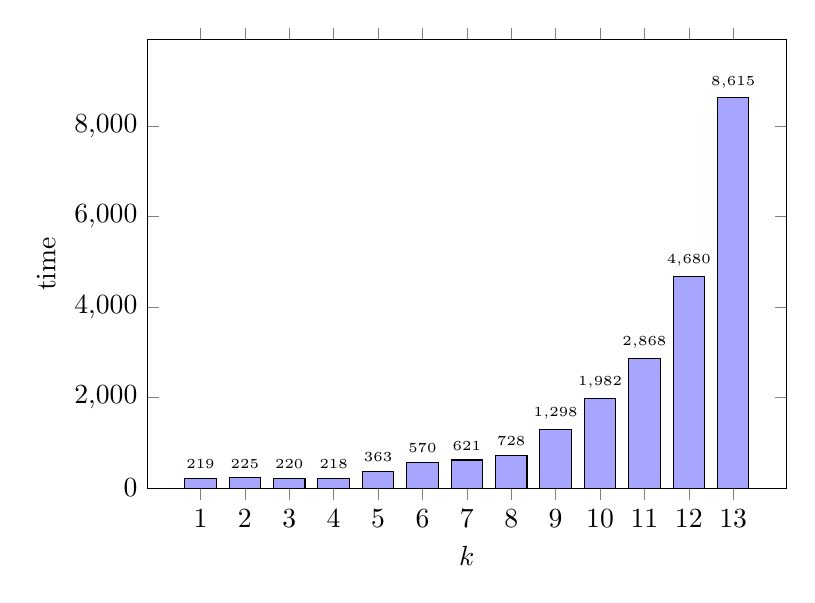
\begin{tikzpicture}
\begin{axis}[
    ybar,
    bar width=0.4cm,
    xlabel=$k$,
    ylabel={time},
    ymin=0,
    ymax=9900,
    xtick=data,
    xticklabels={1,2,3,4,5,6,7,8,9,10,11,12,13},
    width=0.8\textwidth,
    height=0.6\textwidth,
]
\addplot[
    nodes near coords,
    nodes near coords align={vertical},
    nodes near coords style={font=\tiny},
    fill=blue!35, % sets the fill color of the bars to blue
] coordinates {
    (1, 219)
    (2, 225)
    (3, 220)
    (4, 218)
    (5, 363)
    (6, 570)
    (7, 621)
    (8, 728)
    (9, 1298)
    (10, 1982)
    (11, 2868)
    (12, 4680)
    (13, 8615)
};
\end{axis}
\end{tikzpicture}
\end{document}
